\documentclass[11pt,a4paper]{article}
\usepackage[utf8]{inputenc}
\usepackage[T1]{fontenc}
\usepackage{lmodern}
\usepackage[margin=2.5cm]{geometry}
\usepackage{graphicx}
\usepackage{longtable}
\usepackage{array}
\usepackage{amsmath}
\usepackage{amssymb}
\usepackage{microtype}
\usepackage{csquotes}
\usepackage[hidelinks,
  pdftitle={Beyond Market Data: Does Point-in-Time Public Context Add Incremental Predictive Signal?},
  pdfauthor={Ricardo H. Ramos Silva},
  pdfsubject={Working paper (draft)},
  pdfkeywords={point-in-time data, look-ahead bias, pre-registration, cryptocurrency delisting, public context, out-of-time evaluation}]{hyperref}
\setlength{\parskip}{0.5em}
\setlength{\parindent}{0pt}

%% Generated from paper.md by Contextual Alpha/paper/scripts/build_release.py - do not edit by hand.
%% Edit paper.md and regenerate, so the two versions cannot diverge.

\title{Beyond Market Data: Does Point-in-Time Public Context Add Incremental Predictive Signal?\\[6pt]\large A pre-registered, staged test on Binance full-asset delistings}
\author{Ricardo H. Ramos Silva\\[2pt]\textit{Independent Researcher}}
\date{October 2026}
\emergencystretch=3em
\begin{document}
\maketitle
\begin{center}\fbox{\parbox{0.9\linewidth}{\centering\small Working-paper draft, pre-referee. Not peer-reviewed, not submitted, no DOI. Prospective confirmation pending.}}\end{center}

\section*{Abstract}

A common proposal in event-driven research is to add news, regulatory and macroeconomic context to market data, on the premise that public information known at decision time is predictive. Testing that premise requires two conditions that are easy to violate. Context must be reconstructed as it was available at each historical decision time, and it must be transformed into features without importing later knowledge. We test the premise in a staged design that separates the two conditions from the prediction question:

\begin{enumerate}
\item a data-feasibility gate asks which context layers can be reconstructed point-in-time (PIT);
\item a representation gate asks which reconstructed context can become deterministic, auditable, transform-time-PIT features;
\item a pre-registration freezes the predictive comparison before any outcome is opened;
\item the outcome is opened once.
\end{enumerate}

The application is the prediction of Binance full-asset delisting announcements within 365 days. Of five candidate context layers, three were reconstructible and only conditionally so: macro, US political/regulatory, and a thin crypto-systemic layer. Exchange-specific and asset-specific context failed the data gate. Of 25 representations built from the surviving substrate, 18 passed the representation gate. No model-based text representation qualified as transform-time PIT.

In the frozen primary comparison (L2 logistic, $\lambda$ = 10), adding the 18 context features to a 23-feature market baseline did not improve out-of-time precision--recall performance:

\begin{itemize}
\item \textbf{development:} pooled out-of-fold PR-AUC 0.2300 for the market baseline (M0) against 0.2205 with context (M2), $\Delta$PR-AUC $-$0.0095. Two of eight folds were positive, and the two-way cluster-bootstrap 95\% interval was [$-$0.0621, +0.0405];
\item \textbf{locked 2025 block} (not seen by any context model): 0.3270 against 0.3029, $\Delta$ $-$0.0240.
\end{itemize}

The pre-registered verdict is \textbf{PRE-REGISTERED NULL}. Under the frozen point-in-time specification, the surviving public-context feature set did not provide evidence of incremental out-of-time predictive information about Binance full-asset delisting beyond the structured market baseline. Both point estimates were negative, and the development interval included zero. The result concerns that surviving representation, not public context in general.

\section*{1. Introduction}

Market data are the default substrate of quantitative finance. A recurring proposal is that public context, such as macroeconomic releases, regulatory actions and crypto-market news, adds information that prices and volumes do not yet carry. Testing that proposal historically demands more than a model comparison. A feature computed for a past date must use only what was public at that date, and the procedure that turns documents into features must not use knowledge acquired later. Both requirements can fail silently. A current web page about a past day may contain later revisions. A missing source may be coded as "no event". A text representation fitted on a corpus that includes later years can encode the future in its parameters even when every input document is old.

This paper reports a full research cycle built to keep those failures out of a confirmatory test. The cycle is staged so that each stage can fail without contaminating the next:

\begin{itemize}
\item \textbf{H20.0} asks whether context can be reconstructed point-in-time.
\item \textbf{H20.1} asks whether the reconstructed substrate can be represented without future knowledge.
\item \textbf{H20.2} freezes the predictive experiment before any outcome is opened.
\item \textbf{H20.3} opens the outcome once and executes the frozen comparison.
\end{itemize}

The prediction task is deliberately concrete: whether a listed asset on Binance spot receives an official full-asset delisting announcement within the next 365 days. That task has a validated event universe and an established market baseline from prior work in the same repository. It also has a plausible role for context: regulatory pressure, macro conditions and crypto-market stress could precede venue decisions. Binance's current delisting FAQ lists legal/compliance, project going-concern, market and ethical risk among the factors it considers (Binance n.d.). That page is current documentation; it does not establish which criteria applied in each year of the sample.

The answer is a pre-registered null for the context that survived the gates. We report it as a result. We also report precisely what was \emph{not} tested. The context layers arguably closest to the outcome, exchange-specific and asset-specific information, failed the point-in-time data gate and never entered the predictive experiment. That limitation is a finding of the feasibility stage, not an omission.

\textbf{Relation to the companion paper.} This is the second paper from the research programme that produced \emph{Before the Backtest} (Ramos Silva 2026). The two papers share their event data and their discipline. Both use the same validated universe of 201 Binance full-asset delisting events (stage H18.1b), and both fix a design and check its feasibility before any outcome is opened. They ask different questions. \emph{Before the Backtest} asks whether a matched event study has enough common support to be run at all, and stops one that does not. This paper asks whether point-in-time public context adds predictive information to a market baseline. An earlier market-only test on the same delisting target, H18.3, is listed in that paper's research registry, also as a pre-registered null. This paper is a separate study: it does not revise the companion paper, and none of its results is reported there.

\section*{2. Research question and contributions}

\textbf{Question.} Does public context that was genuinely available at a historical decision time add incremental out-of-time predictive information beyond structured market data? The scientific object is the increment $\Delta$PR-AUC = PR-AUC(M2) $-$ PR-AUC(M0), not the absolute performance of either model.

\textbf{Contributions.} They are stated conservatively, and none is claimed as new (see \S{}2.1):

\begin{enumerate}
\item \textbf{Two kinds of point-in-time validity.} We distinguish \emph{document-time} PIT (the source record was public by \emph{t}) from \emph{transform-time} PIT (the transformation injects no knowledge unavailable at \emph{t}). We operationalise the second as a classification of every candidate transform before use. The underlying risk, that a model trained on later text carries later knowledge into historical features, is established in the literature on look-ahead bias in language models (Glasserman and Lin 2023; Kelly et al. 2026).
\item \textbf{A staged design} (source reconstruction $\rightarrow$ representation audit $\rightarrow$ pre-registration $\rightarrow$ outcome opening), with closed verdict lists, frozen bars and hash-chained freezes at each stage. It applies the principle that a design is fixed before outcomes are examined (Rubin 2008; Journal of Behavioral and Experimental Finance n.d.).
\item \textbf{An empirical case study} in which additional public context, reconstructed strictly point-in-time, did not provide evidence of incremental out-of-time predictive value over a market baseline.
\item \textbf{A documentation of the small effective sample of shared context.} Context that is identical for every asset in a week is informed by the number of distinct weeks, not by the number of asset-week rows.
\end{enumerate}

\subsection*{2.1 Related work}

\textbf{Public context and crypto outcomes.} The evidence is mixed and mostly concerns returns, volume or volatility over horizons of hours to days, not 365-day delisting:

\begin{itemize}
\item Regulatory news moves crypto prices, most strongly news about legal status, while unspecific official warnings had no measurable effect (Auer and Claessens 2018). That study measures contemporaneous market reactions, not prediction.
\item Tweet counts predicted next-day trading volume and realised volatility, with weaker and mixed evidence for returns (Shen et al. 2019).
\item Twitter activity and sentiment predicted short-horizon altcoin returns in a short sample, for a selected subset of coins, with low out-of-sample fit (Steinert and Herff 2018).
\item The closest delisting study builds Binance delisting models whose predictors include news counts and topics and social-media metrics (Yang and Kwon 2026). Related distress and dead-coin prediction work uses market and activity variables (B\k{e}dowska-S\'{o}jka et al. n.d.; Fantazzini 2022; Aldhahi and Alsamaani 2026).
\end{itemize}

\textbf{Look-ahead in text representations.} Language models trained on unrestricted corpora can embed information from after a document's date. This look-ahead bias has been assessed for LLM sentiment scores of news headlines (Glasserman and Lin 2023). It is the motivation for point-in-time language models trained only on text available up to each date (Kelly et al. 2026). Our transform-time classification applies the same concern to every representation, including fitted statistics such as TF-IDF, before any feature is used.

\textbf{Real-time information sets.} Using the data vintage available at the decision date, rather than later revised data, is standard in real-time macroeconomics (Croushore and Stark 1999) and is what the ALFRED archive supports (Federal Reserve Bank of St. Louis n.d.).

\textbf{Design discipline.} Fixing the design before outcomes (Rubin 2008; Journal of Behavioral and Experimental Finance n.d.) and accounting for selection across specifications (Bailey and L\'{o}pez de Prado 2014) inform the pre-registration. Our previous paper applied an outcome-free feasibility stop to a related delisting event set (Ramos Silva 2026).

\section*{3. Why historical context is hard to reconstruct}

Four failure modes motivated the design. Each was measured in H20.0 or H20.1 rather than assumed.

\begin{itemize}
\item \textbf{Current version $\neq$ historical version.} Wikipedia's Current-Events day pages are a natural historical record, but they are edited after the fact. On the H20.0 sample, 13.5\% of the items present on today's pages were absent at the decision time, and 96.4\% of the pages were edited after it. Reading the revision current at \emph{t} avoids this; reading today's page does not.
\item \textbf{Missing $\neq$ zero.} A source that was not reachable is not a source that reported nothing. The CFTC press-release surface returned HTTP 429 for 2021--2026 in H20.0. Coding those years as "no CFTC release" would have manufactured a regulatory lull.
\item \textbf{Coverage $\neq$ meaning.} A keyword tag can deliver high coverage and still not mean what its name says. The inherited GDELT crypto tag reached every sampled week, but only 0.679 of its positives were crypto articles when audited (H20.1).
\item \textbf{Transform-time leakage.} A 2020 document embedded by a model trained on 2026 text is a 2020 input passed through a 2026 function. Whether such a representation is a clean historical feature is a separate question from whether the document was public in 2020.
\end{itemize}

These distinctions are related to known concerns about leakage in machine-learning-based science (Kapoor and Narayanan 2023) and selection effects in backtesting (Bailey and L\'{o}pez de Prado 2014). They are also related to the principle that observational designs should be fixed before outcome data are examined (Rubin 2008).

\section*{4. Point-in-time context framework}

\textbf{Layers.} Context is organised by \emph{who the information is about}:

\begin{itemize}
\item \textbf{C1 macro;}
\item \textbf{C2 political/regulatory;}
\item \textbf{C3 crypto-systemic;}
\item \textbf{C4 exchange-specific;}
\item \textbf{C5 asset-specific.}
\end{itemize}

\textbf{Times and admissibility.}

\begin{itemize}
\item Every record carries a public-availability time derived by fixed rules.
\item Day-only documents are admitted from the next local midnight.
\item Macro data vintages are admitted from the end of their vintage date in US Eastern time, so a model sees only the vintage available at \emph{t} (Croushore and Stark 1999; Federal Reserve Bank of St. Louis n.d.).
\item GDELT GKG records are produced in 15-minute update batches, with themes and tone assigned by GDELT's own processing (The GDELT Project 2015). As our own conservative rule, a GDELT 15-minute file is admitted 15 minutes after its stamp.
\item A Wikipedia page is read at the revision current at \emph{t}.
\item A record is admissible at \emph{t} if and only if its availability time is $\leq$ \emph{t}. Information at \emph{t} + 1 minute is future information.
\end{itemize}

\textbf{Document-time versus transform-time PIT.} Document-time PIT is a property of inputs. Transform-time PIT is a property of the mapping from inputs to features, and has three classes:

\begin{itemize}
\item \textbf{PIT\_\allowbreak{}SAFE:} deterministic rules whose parameters were fixed without reference to post-\emph{t} documents. This covers counts, publisher categories, fixed dictionaries of generic terms, fixed arithmetic on as-of vintages, and attributes computed by a publisher at ingest time.
\item \textbf{NON\_\allowbreak{}PIT:} any model or statistic fitted on a corpus that includes post-\emph{t} documents. For language models this is the look-ahead risk documented by (Glasserman and Lin 2023) and (Kelly et al. 2026).
\item \textbf{UNRESOLVED:} plausibly safe but not demonstrated.
\end{itemize}

Only PIT\_\allowbreak{}SAFE features may enter a confirmatory design.

\textbf{Governance.}

\begin{itemize}
\item Every outbound request is logged and refused if it contains outcome vocabulary.
\item Raw bytes are write-once.
\item Every stage freezes its plan and rules before evaluation, records hashes, and logs every departure as a deviation.
\item Verdicts come from closed lists. A criterion that could not be measured is not passed.
\end{itemize}

\section*{5. Context data feasibility (H20.0)}

H20.0 asked whether a sufficiently complete, timestamped, reproducible point-in-time context corpus could be reconstructed. It drew 35 quarterly decision timestamps (2018-Q1 to 2026-Q3) and registered 32 candidate sources, including rejected ones. It collected 141,751 documents for the sample windows, and tested each layer against frozen bars:

\begin{itemize}
\item coverage;
\item year span;
\item timestamp quality;
\item version quality, i.e. the share of documents whose content as of \emph{t} is reconstructible (bar $\geq$ 0.70);
\item refetch reproducibility;
\item licensing;
\item entity resolution for C4 and C5 (bar $\geq$ 0.80).
\end{itemize}

\textbf{Table 1. Context layers and H20.0 data-gate status}

\begin{center}
\footnotesize
\setlength{\tabcolsep}{4pt}
\begin{tabular}{>{\raggedright\arraybackslash}p{0.147\linewidth}>{\raggedright\arraybackslash}p{0.118\linewidth}>{\raggedright\arraybackslash}p{0.132\linewidth}>{\raggedright\arraybackslash}p{0.135\linewidth}>{\raggedright\arraybackslash}p{0.239\linewidth}>{\raggedright\arraybackslash}p{0.159\linewidth}}
\hline
\textbf{layer} & \textbf{G4 version share} & \textbf{G7 entity resolution} & \textbf{failed criteria} & \textbf{severe biases} & \textbf{H20.0 status} \\
\hline
C1 Macro & 0.986 & n/a & none & archive\_\allowbreak{}captured\_\allowbreak{}le\_\allowbreak{}t:S\_\allowbreak{}FED\_\allowbreak{}PRESS & CONDITIONAL (reconstructible) \\
C2 Political / regulatory & 0.875 & n/a & none & archive\_\allowbreak{}captured\_\allowbreak{}le\_\allowbreak{}t:S\_\allowbreak{}FED\_\allowbreak{}PRESS & CONDITIONAL (reconstructible) \\
C3 Crypto-systemic & 1.0 & n/a & none & language\_\allowbreak{}crypto\_\allowbreak{}tag\_\allowbreak{}rate; archive\_\allowbreak{}captured\_\allowbreak{}le\_\allowbreak{}t:S\_\allowbreak{}GDELT\_\allowbreak{}GKG & CONDITIONAL (reconstructible) \\
C4 Exchange-specific & 0.385 & 0.795 & G4\_\allowbreak{}version, G7\_\allowbreak{}entity & archive\_\allowbreak{}captured\_\allowbreak{}le\_\allowbreak{}t:S\_\allowbreak{}BINANCE\_\allowbreak{}CMS & DATA-GATE FAIL / UNTESTED \\
C5 Asset-specific & 0.398 & 0.581 & G4\_\allowbreak{}version, G7\_\allowbreak{}entity & archive\_\allowbreak{}captured\_\allowbreak{}le\_\allowbreak{}t:S\_\allowbreak{}BINANCE\_\allowbreak{}CMS; entity\_\allowbreak{}popularity\_\allowbreak{}any\_\allowbreak{}doc\_\allowbreak{}w30 & DATA-GATE FAIL / UNTESTED \\
\hline
\end{tabular}
\end{center}

\textbf{Verdict: PARTIAL PASS.}

\begin{itemize}
\item \textbf{C1 macro:} reconstructible, conditional on temporal and archive bias.
\item \textbf{C2 political/regulatory:} reconstructible, conditional, and US-only.
\item \textbf{C3 crypto-systemic:} reconstructible only in a limited form, as metadata and structured records, conditional on archive and language bias. The English crypto tag fired on 0.54\% of English GDELT records against 0.14\% of translingual records.
\item \textbf{C4 exchange-specific:} failed. Binance notice text could be shown to read the same at \emph{t} for only 0.385 of documents.
\item \textbf{C5 asset-specific:} failed on version quality (0.398) and point-in-time naming (0.581).
\end{itemize}

Both C4 and C5 are \textbf{DATA-GATE FAIL / UNTESTED}, which is a statement about the data, not an economic rejection.

\section*{6. Representation feasibility (H20.1)}

H20.1 asked whether the C1--C3 substrate could become stable, reproducible, auditable features without future knowledge. It froze its representation rules before drawing an independent evaluation sample of 105 monthly decision timestamps (2018-01 to 2026-09). It then built 25 features in four families:

\begin{itemize}
\item \textbf{R1:} event flags;
\item \textbf{R2:} counts and intensities;
\item \textbf{R3:} text-derived representations;
\item \textbf{R4:} as-of macro values.
\end{itemize}

\textbf{Transform-time audit.} Current LLM extraction, current sentence embeddings and TF-IDF fitted on the full corpus were classified NON\_\allowbreak{}PIT. TF-IDF refitted at each \emph{t}, TF-IDF on a frozen pre-2018 corpus, and pre-2018 static word embeddings were classified UNRESOLVED. None was built. The only R3 feature built was a tone score computed by GDELT at ingest time. Point-in-time language models trained only on earlier text (Kelly et al. 2026) are a possible future route for R3; none was evaluated here.

\textbf{Integrity.}

\begin{itemize}
\item 0 point-in-time violations over 55,561 provenance records;
\item byte-identical deterministic rebuilds;
\item complete provenance;
\item missing values never encoded as zero.
\end{itemize}

\textbf{Semantic audit.} An independent sample of 272 documents was audited against a frozen bar of precision $\geq$ 0.90. The labels were produced by the AI research agent, not by a human. That limitation is disclosed throughout, and no classifier was retuned.

\begin{itemize}
\item The SEC, Federal Register, enforcement, FOMC and Wikipedia classifiers met the bar.
\item The GDELT crypto tag did not: precision 0.679, mostly from articles that mention crypto only in passing.
\item The crypto-stress dictionary had no positives at all in the evaluation windows.
\end{itemize}

\textbf{Table 2. Representation families and H20.1 eligibility}

\begin{center}
\footnotesize
\setlength{\tabcolsep}{4pt}
\begin{tabular}{>{\raggedright\arraybackslash}p{0.101\linewidth}>{\raggedright\arraybackslash}p{0.205\linewidth}>{\raggedright\arraybackslash}p{0.092\linewidth}>{\raggedright\arraybackslash}p{0.116\linewidth}>{\raggedright\arraybackslash}p{0.416\linewidth}}
\hline
\textbf{family} & \textbf{H20.1 verdict} & \textbf{built} & \textbf{eligible} & \textbf{ineligible (criterion)} \\
\hline
R1 & PARTIAL PASS & 6 & 4 & F24: REDUNDANT with F23 (rho 0.9996); F25: semantic defect K5; SPARSE\_\allowbreak{}DEGENERATE (nonzero share 0.0) \\
R2 & PARTIAL PASS & 15 & 11 & F17: coverage 0.314, 4 years; F19: semantic defect K6; F20: semantic defect K6; F21: semantic defect K6 \\
R3 & DATA-GATE FAIL / UNTESTED & 1 & 0 & F22: semantic defect K6 \\
R4 & PASS & 3 & 3 & none \\
\hline
\end{tabular}
\end{center}

\begin{center}
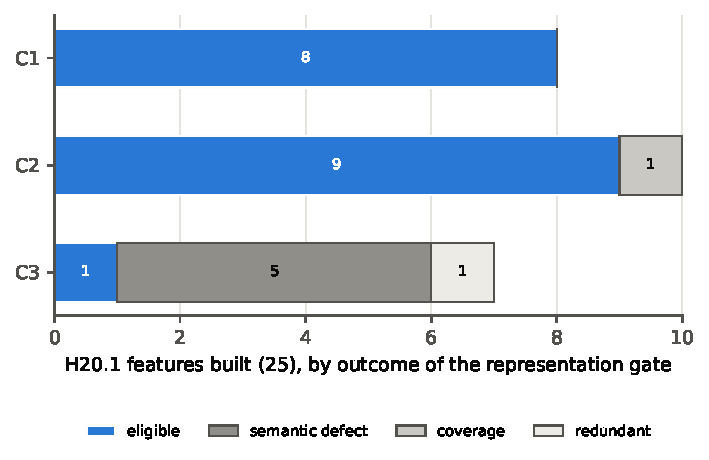
\includegraphics[width=\linewidth]{paper/figures/figure6_feature_survival.pdf}
\end{center}

\emph{Figure 6. H20.1 feature survival by context layer. Of 25 features built, 18 were eligible; C3 lost every GDELT feature to the semantic audit.}

\textbf{Verdict: PARTIAL PASS.}

\begin{itemize}
\item \textbf{R4:} PASS.
\item \textbf{R1, R2:} PARTIAL PASS.
\item \textbf{R3:} DATA-GATE FAIL / UNTESTED.
\end{itemize}

The 18 eligible features are:

\begin{itemize}
\item 8 in C1 (Fed releases and FOMC statements; CPI and unemployment release flags; the as-of policy rate, CPI inflation and unemployment);
\item 9 in C2 (Federal Register financial-regulator and crypto documents; SEC releases, enforcement and crypto releases; Fed enforcement; a crypto regulatory-action flag);
\item 1 in C3.
\end{itemize}

The single C3 survivor is \textbf{generic English-Wikipedia crypto attention}: a count of crypto items on the Current-Events pages. It is not a systemic-crypto-state variable.

\begin{center}
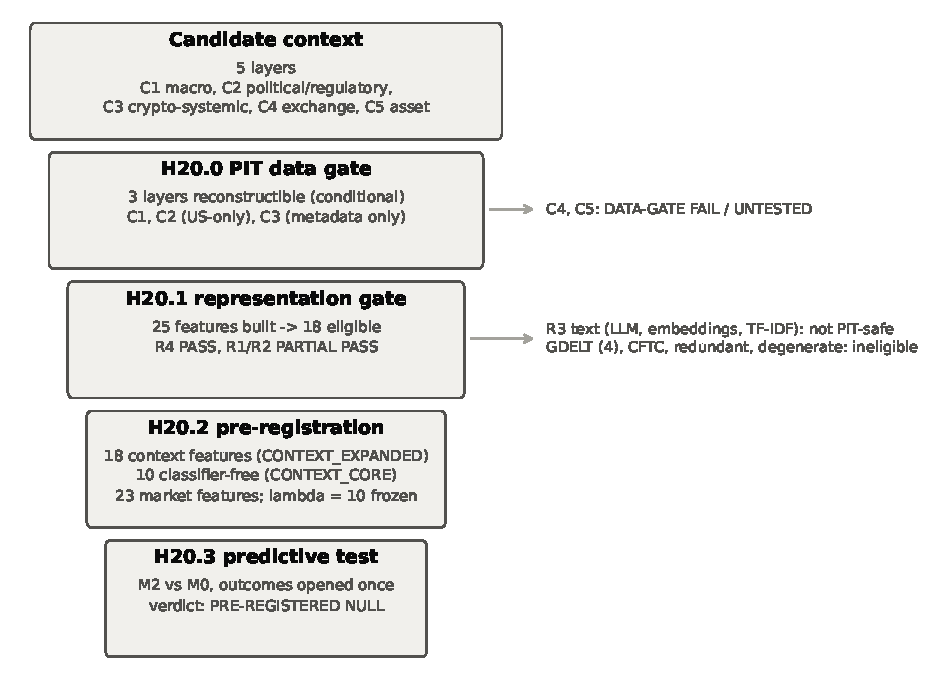
\includegraphics[width=\linewidth]{paper/figures/figure1_research_funnel.pdf}
\end{center}

\emph{Figure 1. The Contextual Alpha research funnel. Each stage could fail independently; C4/C5 and the text representations dropped out before any outcome was opened.}

\section*{7. Pre-registered predictive design (H20.2)}

H20.2 froze the predictive experiment before any outcome was opened. It was hash-chained to the H20.1 freeze and amended once (Addendum 02), before outcomes, as follows:

\begin{itemize}
\item it fixed the primary penalty a priori;
\item it renamed the 2025 block;
\item it made the calibration criterion machine-readable.
\end{itemize}

\textbf{Unit and decision time.} The unit is an asset-era $\times$ weekly landmark. The asset-era follows the inherited rule that a ticker starts a new era only after more than 365 days with no served route. The decision time is \textbf{Tuesday 00:00 UTC after the landmark Monday}, so the landmark day's daily candle is complete at \emph{t}. The design is landmark-style: at each landmark, the risk set is the assets still at risk, and predictors use only information available at the landmark, as in landmarking for dynamic prediction (Putter and van Houwelingen 2017). We model a binary 365-day outcome with logistic regression; no survival model is fitted.

\textbf{Target.} y = 1 if and only if the asset-era's validated full-asset delisting \emph{announcement} falls in (\emph{t}, \emph{t} + 365 days]. The announcement time comes from the frozen event universe and is never the trading end. Landmarks whose announcement was already public at \emph{t} are excluded from the risk set.

\textbf{Features.}

\begin{itemize}
\item \textbf{M0 (23 market features):} liquidity, volatility and trailing return; route state (active pairs, quote assets); venue regime (listed assets, removal intensity, a calendar trend); and route history.
\begin{itemize}
\item Inherited route-history features that rest on a class taken from Binance notice titles (C4) were excluded and replaced by notice-free versions, so the market baseline contains no venue-notice input.
\item Current listing status, whole-era quantities and every outcome column were excluded.
\end{itemize}
\item \textbf{CONTEXT\_\allowbreak{}EXPANDED:} the 18 H20.1-eligible features, computed at every landmark with the unchanged H20.1 rules.
\item \textbf{CONTEXT\_\allowbreak{}CORE:} the 10 features that use no agent-audited text classifier, fixed before any outcome as a robustness set.
\end{itemize}

\textbf{Arms.}

\begin{itemize}
\item \textbf{M0:} market only;
\item \textbf{M2:} market + CONTEXT\_\allowbreak{}EXPANDED;
\item \textbf{M1:} context only;
\item \textbf{M1\_\allowbreak{}core, M2\_\allowbreak{}core:} robustness arms.
\end{itemize}

The primary comparison is \textbf{M2 versus M0}.

\textbf{Model.} L2-penalised logistic regression with a single a-priori $\lambda$ = 10, identical for every arm. The objective is $\Sigma$ log-loss + $\tfrac{1}{2}$$\lambda$$\Vert$$\beta$$\Vert$$^{2}$ on standardised features. Preprocessing is identical for all arms:

\begin{enumerate}
\item a fixed transform per feature;
\item winsorisation at the training 0.5th and 99.5th percentiles;
\item training-median imputation with missing indicators;
\item standardisation.
\end{enumerate}

There is no class weighting and no recalibration. The $\lambda$ grid and a LightGBM model were frozen as \emph{exploratory} only, unable to determine the verdict.

\textbf{Temporal design.}

\begin{itemize}
\item \textbf{Development:} landmarks 2018-01-01 to 2023-12-25, with eight rolling-origin folds (Hyndman and Athanasopoulos 2021). Each fold has an expanding training window, a 365-day embargo and a quarterly test window in 2022--2023. The embargo follows from the label: a training landmark's 365-day outcome window must end before its fold's test window begins, so no delisting event can label both a training row and a test row.
\item \textbf{Embargo:} a one-year embargo follows development.
\item \textbf{LCUV:} a single locked block of landmarks 2025-01-06 to 2025-10-06, called the LOCKED\_\allowbreak{}CONTEXT\_\allowbreak{}UNSEEN\_\allowbreak{}VALIDATION (LCUV) block.
\begin{itemize}
\item No context or H20 model had seen it, and every rule was frozen before H20 scoring.
\item It is \emph{not} an untouched holdout: the earlier H18.3 programme had observed market-only model behaviour in that period.
\end{itemize}
\item \textbf{PROSPECTIVE\_\allowbreak{}CONFIRMATION:} landmarks 2025-10-13 to 2026-09-28. It is the only block untouched by the programme and remains unopened until its outcomes mature.
\end{itemize}

\begin{center}
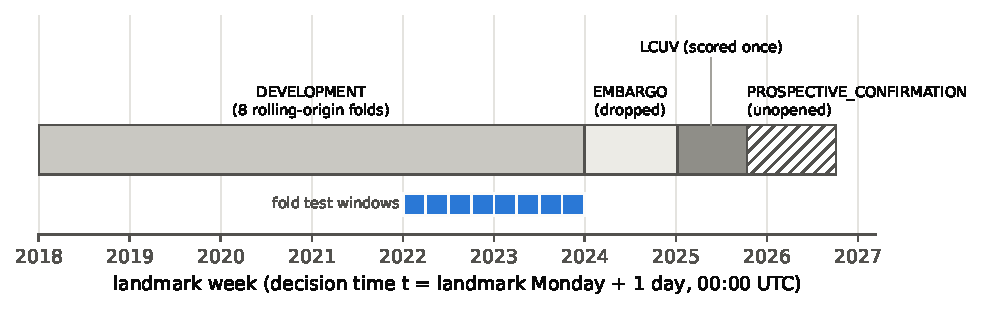
\includegraphics[width=\linewidth]{paper/figures/figure2_timeline.pdf}
\end{center}

\emph{Figure 2. Temporal design. Decision time is the end of each landmark Monday; the prospective block is unopened.}

\textbf{Metrics and inference.}

\begin{itemize}
\item \textbf{Primary:} PR-AUC (average precision), because the positive class is rare and ROC-based summaries can be misleading under heavy class imbalance (Saito and Rehmsmeier 2015).
\item \textbf{Secondary:} ROC-AUC, Brier score, within-week top-decile lift and calibration.
\item \textbf{Uncertainty:} a 2,000-replicate two-way bootstrap on the fixed out-of-fold predictions.
\begin{itemize}
\item It adapts the pigeonhole bootstrap (Owen 2007), which resamples the row entities and the column entities of a crossed design independently, with replacement. Here the rows are asset-eras and the columns are the eight fold test windows (quarterly calendar blocks), not individual weeks. Each landmark row is weighted by the product of its asset-era and block multiplicities, and the statistic is a weighted PR-AUC difference.
\item Owen's consistency results concern means, and Owen describes the procedure as mildly conservative there. For a rank-based statistic such as PR-AUC they are an approximation, not a guarantee.
\item Rows are clustered because observations of one asset and of one period are correlated, and ignoring that correlation biases conventional standard errors (Petersen 2006).
\end{itemize}
\end{itemize}

\textbf{Promotion rule.} Support requires all of S1--S7:

\begin{itemize}
\item \textbf{S1:} positive development $\Delta$;
\item \textbf{S2:} at least five of eight positive folds;
\item \textbf{S3:} a bootstrap lower bound above zero;
\item \textbf{S4:} a positive LCUV $\Delta$;
\item \textbf{S5:} no severe calibration deterioration;
\item \textbf{S6:} a clean PIT audit;
\item \textbf{S7:} a result not driven by one era.
\end{itemize}

The closed verdict list is INCREMENTAL CONTEXT SIGNAL SUPPORTED, PRE-REGISTERED NULL, NEGATIVE INCREMENTAL RESULT and DATA / DESIGN FAILURE.

\section*{8. Empirical results (H20.3)}

\subsection*{8.1 Execution and audits}

H20.3 followed the frozen P0--P6 sequence.

\begin{itemize}
\item \textbf{Context at every landmark} (353 decision times $\times$ 18 features):
\begin{itemize}
\item zero records available after \emph{t} and zero post-\emph{t} joins;
\item complete provenance;
\item byte-identical deterministic rebuilds.
\end{itemize}
\item \textbf{Route-state fallback.} The pre-registered structural trigger fired: window-based and candle-based route states disagreed on 4.554\% of landmarks, above the frozen 1\% bar. The frozen candle-based fallback was therefore applied. This was a structural rule computed before any outcome, not a post-result change.
\item \textbf{X sealed before the outcome.} The feature matrix was sealed and hashed before the lifecycle table was opened.
\item \textbf{Target.}
\begin{itemize}
\item Strict timestamp parsing found no failures, and no event matched more than one asset-era.
\item The independently rebuilt target agreed with the inherited H18 label on all 93,394 matched rows.
\end{itemize}
\item \textbf{Primary LCUV scoring} ran exactly once.
\end{itemize}

The PIT, target and execution audits all passed.

\subsection*{8.2 Effective sample}

\textbf{Table 3. Temporal design and effective sample size}

\begin{center}
\scriptsize
\setlength{\tabcolsep}{1.5pt}
\begin{tabular}{>{\raggedright\arraybackslash}p{0.196\linewidth}>{\raggedright\arraybackslash}p{0.162\linewidth}>{\raggedright\arraybackslash}p{0.119\linewidth}>{\raggedright\arraybackslash}p{0.105\linewidth}>{\raggedright\arraybackslash}p{0.074\linewidth}>{\raggedright\arraybackslash}p{0.119\linewidth}>{\raggedright\arraybackslash}p{0.155\linewidth}}
\hline
\textbf{block} & \textbf{landmark Mondays} & \textbf{landmark rows} & \textbf{asset-eras} & \textbf{weeks} & \textbf{unique events} & \textbf{positive landmark rate} \\
\hline
DEVELOPMENT & 2018-01-01 to 2023-12-25 & 78227 & 522 & 313 & 110 & 5.82\% \\
EMBARGO (dropped) & 2024-01-01 to 2024-12-30 & not built &  & 53 &  &  \\
LCUV & 2025-01-06 to 2025-10-06 & 15167 & 443 & 40 & 86 & 11.79\% \\
PROSPECTIVE\_\allowbreak{}CONFIRMATION (unopened) & 2025-10-13 to 2026-09-28 & not built &  & 51 &  &  \\
\hline
\end{tabular}
\end{center}

Positive landmark rows are not independent events. One delisting is the label of up to 52 consecutive weekly landmarks. Development contains 110 unique events, and the out-of-fold evaluation spans 104 distinct weeks. Because context is common to every asset in a week, its evidence rests on those weeks rather than on the 78,227 development rows.

\subsection*{8.3 Primary result}

\textbf{Table 4. Development pooled out-of-fold results (L2 logistic, lambda = 10)}

\begin{center}
\scriptsize
\setlength{\tabcolsep}{1.5pt}
\begin{tabular}{>{\raggedright\arraybackslash}p{0.168\linewidth}>{\raggedright\arraybackslash}p{0.099\linewidth}>{\raggedright\arraybackslash}p{0.076\linewidth}>{\raggedright\arraybackslash}p{0.082\linewidth}>{\raggedright\arraybackslash}p{0.076\linewidth}>{\raggedright\arraybackslash}p{0.168\linewidth}>{\raggedright\arraybackslash}p{0.132\linewidth}>{\raggedright\arraybackslash}p{0.128\linewidth}}
\hline
\textbf{arm} & \textbf{role} & \textbf{PR-AUC} & \textbf{ROC-AUC} & \textbf{Brier} & \textbf{top-decile lift (within-week)} & \textbf{within-week PR-AUC} & \textbf{calibration slope} \\
\hline
M0 market & primary & 0.23 & 0.767 & 0.0512 & 4.51 & 0.247 & 0.67 \\
M2 market + context & primary & 0.2205 & 0.75 & 0.0521 & 4.6 & 0.244 & 0.52 \\
M1 context only & secondary & 0.0674 & 0.54 & 0.0592 & 0.64 & 0.059 & 0.17 \\
M2\_\allowbreak{}core market + CONTEXT\_\allowbreak{}CORE & robustness & 0.2303 & 0.759 & 0.0522 & 4.61 & 0.245 & 0.58 \\
M1\_\allowbreak{}core CONTEXT\_\allowbreak{}CORE only & robustness & 0.0675 & 0.541 & 0.0573 & 0.64 & 0.059 & 0.2 \\
\hline
\end{tabular}
\end{center}

\textbf{Table 5. LOCKED\_\allowbreak{}CONTEXT\_\allowbreak{}UNSEEN\_\allowbreak{}VALIDATION (2025) results, scored once (L2 logistic, lambda = 10)}

\begin{center}
\scriptsize
\setlength{\tabcolsep}{1.5pt}
\begin{tabular}{>{\raggedright\arraybackslash}p{0.168\linewidth}>{\raggedright\arraybackslash}p{0.099\linewidth}>{\raggedright\arraybackslash}p{0.076\linewidth}>{\raggedright\arraybackslash}p{0.082\linewidth}>{\raggedright\arraybackslash}p{0.076\linewidth}>{\raggedright\arraybackslash}p{0.168\linewidth}>{\raggedright\arraybackslash}p{0.132\linewidth}>{\raggedright\arraybackslash}p{0.128\linewidth}}
\hline
\textbf{arm} & \textbf{role} & \textbf{PR-AUC} & \textbf{ROC-AUC} & \textbf{Brier} & \textbf{top-decile lift (within-week)} & \textbf{within-week PR-AUC} & \textbf{calibration slope} \\
\hline
M0 market & primary & 0.327 & 0.809 & 0.0929 & 3.21 & 0.35 & 1.05 \\
M2 market + context & primary & 0.3029 & 0.806 & 0.096 & 3.12 & 0.33 & 0.99 \\
M1 context only & secondary & 0.1193 & 0.506 & 0.1073 & 0.87 & 0.118 & 0.34 \\
M2\_\allowbreak{}core market + CONTEXT\_\allowbreak{}CORE & robustness & 0.3112 & 0.808 & 0.0972 & 3.1 & 0.337 & 1.01 \\
M1\_\allowbreak{}core CONTEXT\_\allowbreak{}CORE only & robustness & 0.1212 & 0.51 & 0.1091 & 0.87 & 0.118 & 1.25 \\
\hline
\end{tabular}
\end{center}

\begin{center}
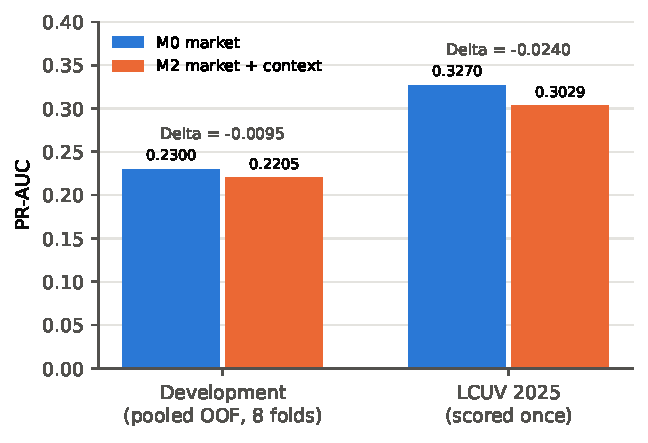
\includegraphics[width=\linewidth]{paper/figures/figure3_primary_pr_auc.pdf}
\end{center}

\emph{Figure 3. Primary PR-AUC, market baseline (M0) versus market + context (M2), in development (pooled out-of-fold) and on the LCUV block.}

\textbf{Development.}

\begin{itemize}
\item Pooled out-of-fold PR-AUC was 0.2300 for M0 and 0.2205 for M2: \textbf{$\Delta$PR-AUC = $-$0.0095}, a relative change of $-$4.1\%.
\item Two of eight folds were positive.
\item The two-way cluster-bootstrap 95\% interval was [$-$0.0621, +0.0405].
\end{itemize}

\textbf{LCUV (scored once).} PR-AUC was 0.3270 for M0 and 0.3029 for M2: \textbf{$\Delta$PR-AUC = $-$0.0240}, relative $-$7.4\%. The informational interval was [$-$0.061, +0.001].

\textbf{Secondary metrics.} ROC-AUC and Brier score moved in the same direction as PR-AUC. Calibration on the LCUV block did not deteriorate severely (Brier ratio 1.033 $\leq$ 1.05; slope excess $-$0.044 $\leq$ 0.20).

\begin{center}
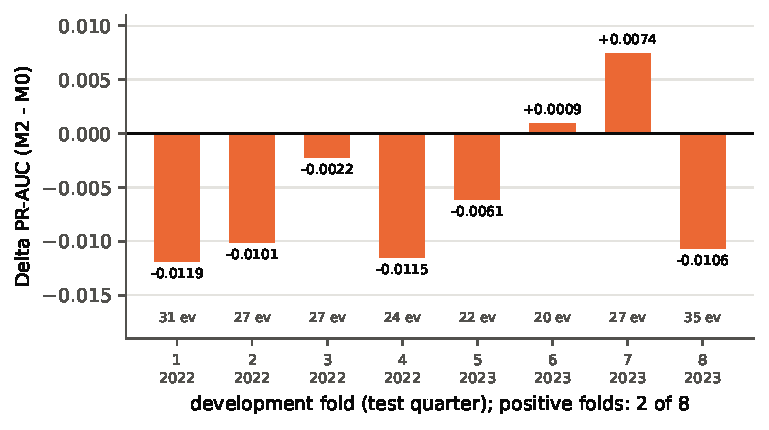
\includegraphics[width=\linewidth]{paper/figures/figure4_fold_delta.pdf}
\end{center}

\emph{Figure 4. Fold-level $\Delta$PR-AUC (M2 $-$ M0) for the eight development folds, with unique test events per fold.}

\begin{center}
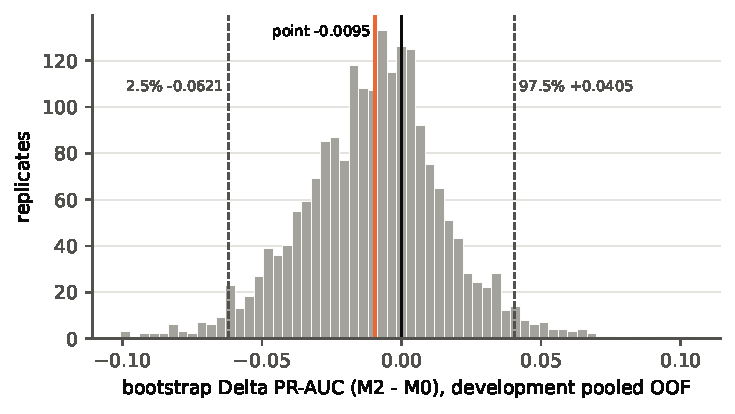
\includegraphics[width=\linewidth]{paper/figures/figure5_bootstrap_delta.pdf}
\end{center}

\emph{Figure 5. Two-way cluster-bootstrap distribution of the development $\Delta$PR-AUC (2,000 replicates); dashed lines mark the 95\% interval.}

\subsection*{8.4 Verdict}

\textbf{Table 6. Pre-registered criteria S1-S7 and the mechanical verdict}

\begin{center}
\small
\setlength{\tabcolsep}{4pt}
\begin{tabular}{>{\raggedright\arraybackslash}p{0.133\linewidth}>{\raggedright\arraybackslash}p{0.394\linewidth}>{\raggedright\arraybackslash}p{0.294\linewidth}>{\raggedright\arraybackslash}p{0.109\linewidth}}
\hline
\textbf{criterion} & \textbf{condition} & \textbf{observed} & \textbf{result} \\
\hline
S1 & development pooled-OOF Delta > 0 & -0.0095 & FAIL \\
S2 & >= 5 of 8 folds with Delta > 0 & 2 of 8 & FAIL \\
S3 & two-way bootstrap 95\% CI lower bound > 0 & [-0.0621, +0.0405] & FAIL \\
S4 & LCUV Delta > 0 & -0.0240 & FAIL \\
S5 & no severe calibration deterioration (Brier ratio <= 1.05; slope excess <= 0.20) & Brier ratio 1.033; slope excess -0.044 & PASS \\
S6 & PIT audit passes & all stages PASS & PASS \\
S7 & >= 2 of 3 era blocks positive and leave-one-fold-out Delta > 0 & 1 of 3 eras positive; min LOFO Delta -0.0143 & FAIL \\
verdict & closed list, applied mechanically & PRE-REGISTERED NULL &  \\
\hline
\end{tabular}
\end{center}

S5 and S6 passed. S1, S2, S3, S4 and S7 failed. No DATA / DESIGN FAILURE condition held: the PIT, target, reproducibility and execution audits passed. The result is not a NEGATIVE INCREMENTAL RESULT, because the development interval's upper bound (+0.0405) is above zero. The mechanical verdict is \textbf{PRE-REGISTERED NULL}.

\section*{9. Robustness and exploratory results}

\textbf{Table 7. Robustness and exploratory results (cannot change the verdict)}

\begin{center}
\footnotesize
\setlength{\tabcolsep}{4pt}
\begin{tabular}{>{\raggedright\arraybackslash}p{0.240\linewidth}>{\raggedright\arraybackslash}p{0.166\linewidth}>{\raggedright\arraybackslash}p{0.146\linewidth}>{\raggedright\arraybackslash}p{0.112\linewidth}>{\raggedright\arraybackslash}p{0.265\linewidth}}
\hline
\textbf{analysis} & \textbf{status} & \textbf{development Delta} & \textbf{LCUV Delta} & \textbf{note} \\
\hline
CONTEXT\_\allowbreak{}CORE (classifier-free), primary lambda & robustness (secondary) & 0.0003 & -0.0158 & two-way CI [-0.042, +0.045]; 3 of 8 folds positive \\
logistic, fold-selected lambda & EXPLORATORY & 0.0273 & -0.0167 & M2 configuration: 1000.0 \\
LightGBM, a-priori default & EXPLORATORY & 0.0285 & -0.008 & M2 configuration: \{'num\_\allowbreak{}leaves': 7, 'n\_\allowbreak{}estimators': 200\} \\
LightGBM, fold-selected & EXPLORATORY & 0.0271 & -0.003 & M2 configuration: \{'num\_\allowbreak{}leaves': 7, 'n\_\allowbreak{}estimators': 200\} \\
\hline
\end{tabular}
\end{center}

\textbf{Classifier-free context (CONTEXT\_\allowbreak{}CORE, secondary).} Replacing the expanded set with the 10 features that use no agent-audited classifier gave:

\begin{itemize}
\item a development $\Delta$ of +0.0003, with a two-way interval of [$-$0.042, +0.045];
\item an LCUV $\Delta$ of $-$0.0158.
\end{itemize}

The null pattern persists in the classifier-free robustness specification. This shows that the pattern is robust to removing those classifiers; it does not show that the classifiers had no influence on the expanded-set result.

\textbf{Exploratory tuning (labelled exploratory; cannot change the verdict).} More flexible or fold-selected models showed apparent development gains that did not persist into the locked block:

\begin{center}
\small
\setlength{\tabcolsep}{4pt}
\begin{tabular}{>{\raggedright\arraybackslash}p{0.449\linewidth}>{\raggedright\arraybackslash}p{0.286\linewidth}>{\raggedright\arraybackslash}p{0.195\linewidth}}
\hline
\textbf{model} & \textbf{development $\Delta$} & \textbf{LCUV $\Delta$} \\
\hline
logistic, fold-selected $\lambda$ & +0.027 & $-$0.017 \\
LightGBM, a-priori configuration & +0.029 & $-$0.008 \\
LightGBM, fold-selected & +0.027 & $-$0.003 \\
\hline
\end{tabular}
\end{center}

More flexible or selected specifications produced apparent development improvements that did not persist in the locked context-unseen block. Each fold-selected configuration was chosen on the same folds that score it, so the pattern is consistent with selection optimism, which the a-priori primary penalty was frozen to avoid. It does not, by itself, identify overfitting.

\textbf{Context-only arms.} Context-only models (M1, M1\_\allowbreak{}core) showed little discrimination: development ROC-AUC 0.540 and 0.541. This is consistent with context ranking weeks rather than assets.

\section*{10. Discussion}

The study did not support the incremental-context hypothesis. The surviving representation, built and audited as it was, did not improve out-of-time predictive performance for this target beyond this baseline. The point estimates were negative, but the development interval included zero and is wide enough that neither a negative nor a moderate positive increment is excluded. Several interpretations are compatible with this finding. None is identified by the experiment, and they are offered as hypotheses, not mechanisms.

\begin{enumerate}
\item \textbf{Redundancy.} Part of the public context may already be reflected in market variables such as liquidity, volatility and route structure, which respond to the same conditions.
\item \textbf{Target mismatch.} Macro and regulatory context can move market-wide risk without discriminating \emph{which} asset will be fully delisted within a year.
\item \textbf{Cross-sectional limitation.} Context is identical for every asset at a given week. In a linear model it adds the same shift to every asset's score in that week, so it cannot by itself reorder assets within a week. The context-only arms' near-chance ROC-AUC is consistent with this.
\item \textbf{Horizon mismatch.} Short-lived public events may be weak predictors of an asset-specific decision up to 365 days later.
\item \textbf{Representation limitation.} The context most plausibly relevant to an asset's delisting, exchange-specific notices and asset-specific information, failed the point-in-time data gate and was never allowed into the confirmatory experiment. Stronger representations of those layers could behave differently.
\end{enumerate}

The exploratory pattern is itself informative for practice. Tuned and more flexible models produced development gains of about +0.03 that reversed sign on the locked block. In a study without a frozen a-priori primary and a locked block, that pattern could have been reported as a context effect.

\section*{11. Limitations}

\begin{itemize}
\item \textbf{Untested context.}
\begin{itemize}
\item C4 and C5 failed the data gate and were not tested.
\item GDELT features failed the semantic audit.
\item No modern LLM, modern embedding or non-PIT text transform was used.
\item The C3 representation is thin: generic English-Wikipedia crypto attention.
\end{itemize}
\item \textbf{Scope of the surviving context.} C2 is US-only. C1--C3 inherit H20.0's archive and language conditions.
\item \textbf{Low power for a week-level signal.} The out-of-fold evaluation spans 104 weeks and the LCUV block 40, with 110 and 86 unique events. A modest true effect would be hard to detect.
\item \textbf{Agent-produced semantic audit.} Eight of the 18 context features depend on classifiers audited by the AI research agent. The null pattern persists in the classifier-free robustness specification.
\item \textbf{The LCUV block} is context-unseen, not programme-untouched. Prospective confirmation is pending.
\item \textbf{Market substrate approximations.} Route state is reconstructed from daily candles; the frozen fallback addressed window gaps. Two events (IDRT, VAI) have no candles and two others (SKY, USDS) attach to no era under the inherited era rule; the rebuilt target agreed with the inherited label on every matched row.
\item \textbf{Single venue and target.} Results concern Binance full-asset delisting announcements and do not extend to other venues, targets or horizons.
\end{itemize}

\section*{12. Implications for event-driven research}

\begin{enumerate}
\item Separate document-time from transform-time point-in-time validity. Classify every transform before use; treat models trained on later corpora as non-PIT by default.
\item Gate context sources before modelling. Let a layer fail as "untested" rather than fill it with current versions or zeros.
\item Report the effective sample of shared context: distinct decision times and unique events, not asset-time rows.
\item Freeze an a-priori primary specification and a locked evaluation block; treat tuned gains as exploratory until they survive the block.
\item Report nulls with their scope. "This representation did not show incremental value here" is a result that a broader claim must not overwrite, and it is not evidence that no effect exists.
\end{enumerate}

\section*{13. Conclusion}

Under the frozen point-in-time specification, the surviving public-context feature set did not provide evidence of incremental out-of-time predictive information about Binance full-asset delisting beyond the structured market baseline. The pre-registered verdict is PRE-REGISTERED NULL. This is an absence of evidence of incremental value, not evidence that context has no effect: the point estimates were negative and the development interval included zero. The finding is bounded by what survived the gates. Exchange-specific and asset-specific context could not be reconstructed point-in-time here and remain untested. Prospective confirmation is pending.

\section*{Data and code availability}

All stages are reproducible from the Contextual Alpha project directory. It contains:

\begin{itemize}
\item frozen plans, pre-registrations and freeze files with SHA-256 hashes;
\item collection, build, audit and model scripts;
\item tests;
\item the evidence tables behind every number.
\end{itemize}

Frozen commits: H20.0 \texttt{a14c347}, H20.1 \texttt{e21c264}, H20.2 with Addendum 02 \texttt{9932e20}, H20.3 \texttt{180def4}. Raw source content is not redistributed. Paper tables and figures are regenerated by \texttt{paper/scripts/build\_\allowbreak{}paper\_\allowbreak{}assets.py}.

\section*{References}

The reference list is \texttt{paper/references.bib}.

\begin{itemize}
\item Eleven entries are reused unchanged from the author's previous paper in the same repository, which is itself cited as (Ramos Silva 2026).
\item Fourteen entries were added in a verification pass. Each was read at the level recorded in \texttt{paper/REFERENCE\_\allowbreak{}VERIFICATION.md}.
\item Remaining gaps are recorded in \texttt{paper/REFERENCE\_\allowbreak{}GAPS.md}.
\end{itemize}

Related work on cryptocurrency delisting and distress prediction includes (Yang and Kwon 2026), (B\k{e}dowska-S\'{o}jka et al. n.d.), (Fantazzini 2022) and (Aldhahi and Alsamaani 2026). Survivorship and delisting bias are covered in (Shumway 1997) and (Ammann et al. 2022). Registered reports and dispersion across analysts are covered in (Journal of Behavioral and Experimental Finance n.d.) and (Menkveld et al. 2024).

Rendered from \texttt{paper/references.bib}, the source of truth. Each entry carries the access level recorded for it in \texttt{paper/REFERENCE\_\allowbreak{}VERIFICATION.md}; no metadata was inferred.

\begin{itemize}
\item \textbf{Aldhahi and Alsamaani} (2026). \emph{Regime-Dependent Predictability of Cryptocurrency Distress: Cross-Sectional Evidence from Two Exchanges}. Journal of Risk and Financial Management 19(8), 599. DOI: 10.3390/jrfm19080599.   \emph{Accessed at abstract level; the publisher returned HTTP 403. Coin-quarter panel that retains coins which later become inactive; panel logit; cross-validated out-of-sample AUC of approximately 0.68. Given names were not recorded by the source consulted and are not supplied here.}
\item \textbf{Ammann, Burdorf, Liebi and St\"{o}ckl} (2022). \emph{Survivorship and Delisting Bias in Cryptocurrency Markets}. University of St. Gallen.   \emph{Retrieved in full. 3,904 cryptocurrencies, January 2014 to December 2021, 417 weeks; 1,222 delisted (39.5 percent). Bias of 0.93 percent annualised value-weighted and 62.19 percent equal-weighted. Attributes the bias to reliance on aggregators that provide historical data only for currently listed assets - the aggregator side of the asymmetry this manuscript measures from the venue side. SSRN record 4287573. Given names were not recorded by the source consulted and are not supplied here.}
\item \textbf{Auer, R. and Claessens, S.} (2018). \emph{Regulating cryptocurrencies: assessing market reactions}. BIS Quarterly Review.   \emph{Full article read on the BIS site (September 2018 issue). Event study of regulatory news.}
\item \textbf{Bailey, D. H. and L\'{o}pez de Prado, M.} (2014). \emph{The Deflated Sharpe Ratio: Correcting for Selection Bias, Backtest Overfitting and Non-Normality}. The Journal of Portfolio Management 40(5), 94--107.   \emph{Accessed at abstract and SSRN-record level (SSRN 2460551). Corrects a reported Sharpe ratio for the number of trials, skewness and kurtosis. Establishes that the count of strategy variants tried is a required input to any performance claim. Cited here as prior work that already owns the "a spectacular backtest is a candidate artefact" message at the model-selection layer.}
\item (n.d.). \emph{Registered Reports: Author Guidelines}. Journal of Behavioral and Experimental Finance.   \emph{Accessed at guidelines-document level. The clearest finance-journal instance of the registered-report format, in which methods and planned analyses are pre-registered and reviewed before the research is conducted, stated as a remedy for publication bias and questionable research practices. Year and editor not recorded by the source consulted and not supplied here.}
\item \textbf{Binance} (n.d.). \emph{Binance Delisting Guidelines \& Frequently Asked Questions}. https:/\allowbreak{}/\allowbreak{}www.binance.com/\allowbreak{}en/\allowbreak{}support/\allowbreak{}faq/\allowbreak{}detail/\allowbreak{}e5a9718ccb794acda1c48db5c71753e4.   \emph{Official documentation, accessed 2026-10-19. The page states it was published 2022-12-19 and updated 2026-06-10. This is the CURRENT version, not a historical one; it does not establish the criteria applied in earlier years.}
\item \textbf{B\k{e}dowska-S\'{o}jka, B., W\'{o}jcik, P. and Pele, D. T.} (n.d.). \emph{Early warning systems for cryptocurrency markets: Predicting `zombie' assets using machine learning}. The North American Journal of Economics and Finance 81. DOI: 10.1016/j.najef.2025.102543.   \emph{Accessed at abstract, SSRN record and RePEc metadata level; the publisher returned HTTP 403. Working paper: SSRN 4942031, August 2024. Reports approximately 84 percent out-of-time balanced accuracy at a 28-day horizon.}
\item \textbf{Croushore, D. and Stark, T.} (1999). \emph{A Real-Time Data Set for Macroeconomists}. Federal Reserve Bank of Philadelphia, Research Department.   \emph{Full text read (working paper). Abstract and Section I. A later journal version is listed by EconPapers; its metadata were not read and it is not cited.}
\item \textbf{Fantazzini} (2022). \emph{Crypto-Coins and Credit Risk}. Journal of Risk and Financial Management 15(7), 304. DOI: 10.3390/jrfm15070304.   \emph{Over 2,000 coins, 2015-2020. Tests several competing definitions of a dead coin; the best model depends on coin age and forecast horizon. The given name, any subtitle and the access level were not recorded by the source consulted and none is claimed here.}
\item \textbf{Glasserman, P. and Lin, C.} (2023). \emph{Assessing Look-Ahead Bias in Stock Return Predictions Generated By GPT Sentiment Analysis}. arXiv:2309.17322.   \emph{Full text read (arXiv v1, HTML), including the Abstract and Sections 1.1 and 2.4. A later journal publication is reported elsewhere but was not verified and is not cited.}
\item \textbf{Hyndman, R. J. and Athanasopoulos, G.} (2021). \emph{Forecasting: Principles and Practice}.   \emph{Section 5.10, "Time series cross-validation", read online, accessed 2026-10-19.}
\item \textbf{Kapoor, S. and Narayanan, A.} (2023). \emph{Leakage and the reproducibility crisis in machine-learning-based science}. Patterns 4(9), 100804. DOI: 10.1016/j.patter.2023.100804.   \emph{Accessed at abstract and project-page level; the three top-level taxonomy categories were read from the authors' project page, the full eight-type taxonomy was not. Surveys 17 fields and 294 affected papers in the published version (329 in the 2022 arXiv preprint, arXiv:2207.07048). Its second top-level category, "model uses features which are not legitimate", plausibly already covers the classification-level leakage this manuscript measures; the manuscript therefore claims a detection procedure and a measured rate, not a new category.}
\item \textbf{Kelly, B. T., Malamud, S., Schwab, J. and Xu, T. A.} (2026). \emph{Scaling Point-in-Time Language Models}. National Bureau of Economic Research.   \emph{Full text read: title page, abstract and introduction. Not peer-reviewed, as the working paper states.}
\item \textbf{Federal Reserve Bank of St. Louis} (n.d.). \emph{Help | ALFRED}. https:/\allowbreak{}/\allowbreak{}alfred.stlouisfed.org/\allowbreak{}help.   \emph{Official documentation, accessed 2026-10-19. Sections "What is ALFRED?" and the release-date sections. Current page.}
\item \textbf{Menkveld, A. J. and others} (2024). \emph{Nonstandard Errors}. The Journal of Finance 79(3), 2339--2390. DOI: 10.1111/jofi.13337.   \emph{Accessed at metadata and repository-record level. Multi-team design: many independent research teams are given the same data and the same hypothesis, and the dispersion of their results is measured. Open access under CC BY. The full author list is very long and is abbreviated here as "and others" rather than guessed. Cited as the prior work that owns researcher-discretion variation; its object is dispersion across analysis choices on a shared dataset, which is downstream of the dataset-construction failures this manuscript documents.}
\item \textbf{Owen, A. B.} (2007). \emph{The pigeonhole bootstrap}. The Annals of Applied Statistics 1(2), 386--411. DOI: 10.1214/07-AOAS122.   \emph{Full text read (arXiv:0712.1111v1 reprint). Section 3.2 defines the method: rows and columns sampled IID with replacement, independently, resampled data = their intersections. Section 4 gives variance results for totals and means; p. 2 calls the procedure mildly conservative.}
\item \textbf{Petersen, M. A.} (2006). \emph{Estimating Standard Errors in Finance Panel Data Sets: Comparing Approaches}. National Bureau of Economic Research.   \emph{Full text read (working paper dated April 2005, revised June 2006): abstract and introduction. The later journal version was not read and is not cited.}
\item \textbf{The GDELT Project} (2015). \emph{The GDELT Global Knowledge Graph (GKG) Data Format Codebook V2.1}. http:/\allowbreak{}/\allowbreak{}data.gdeltproject.org/\allowbreak{}documentation/\allowbreak{}GDELT-Global\_\allowbreak{}Knowledge\_\allowbreak{}Graph\_\allowbreak{}Codebook-V2.1.pdf.   \emph{Official documentation, accessed 2026-10-19. Dated 2/19/2015 on its first page. Pages 1, 6, 8 and 10 cover the introduction, GKGRECORDID (15-minute update batch), V1/V2 themes and the tone field. The PDF metadata name Kalev Leetaru as author; no author is printed on the page.}
\item \textbf{Putter, H. and van Houwelingen, H. C.} (2017). \emph{Understanding Landmarking and Its Relation with Time-Dependent Cox Regression}. Statistics in Biosciences 9(2), 489--503. DOI: 10.1007/s12561-016-9157-9.   \emph{Full text read (open access, PMC5711994; CC BY 4.0). Published online 2016-07-11; issue year 2017. Introduction and Theory sections.}
\item \textbf{Ramos Silva, R. H.} (2026). \emph{Before the Backtest: Pre-Freeze Common-Support Ceilings for Event-Driven Strategy Research}. https:/\allowbreak{}/\allowbreak{}github.com/\allowbreak{}ricardohenrique1609/\allowbreak{}before-the-backtest.   \emph{Version 1.0.0, released 2026-10-13, per the repository CITATION.cff. No DOI has been created. The author's previous paper in the same research repository.}
\item \textbf{Rubin, D. B.} (2008). \emph{For objective causal inference, design trumps analysis}. The Annals of Applied Statistics 2(3). DOI: 10.1214/08-AOAS187.   \emph{Accessed at abstract, arXiv (0811.1640) and Project Euclid record level; the full text was not read. States that observational studies must be designed without examining any outcome data, and that a candidate dataset may have to be rejected as inadequate for lack of covariate data or lack of overlap between treatment and control groups, often revealed by propensity-score analysis. \textbf{This is the design-stage rejection principle that this paper operationalises; the principle is Rubin's and is not claimed here.} Page numbers were not recorded by the source consulted and are not supplied.}
\item \textbf{Saito, T. and Rehmsmeier, M.} (2015). \emph{The Precision-Recall Plot Is More Informative than the ROC Plot When Evaluating Binary Classifiers on Imbalanced Datasets}. PLoS ONE 10(3), e0118432. DOI: 10.1371/journal.pone.0118432.   \emph{Full text read (open access). Abstract, Results and Discussion, Conclusion.}
\item \textbf{Shen, D., Urquhart, A. and Wang, P.} (2019). \emph{Does Twitter predict Bitcoin?}. Economics Letters 174, 118--122. DOI: 10.1016/j.econlet.2018.11.007.   \emph{Full text read (accepted version, University of Reading CentAUR, CC BY-NC-ND). Author names are given as printed by the repository (initials only).}
\item \textbf{Shumway, T.} (1997). \emph{The Delisting Bias in CRSP Data}. The Journal of Finance 52(1), 327--340.   \emph{Accessed at abstract and RePEc-record level. Documents that correct delisting returns are missing for most stocks delisted for negative reasons, so studies that drop delisted firms overstate average returns. The canonical statement of the survivorship problem this manuscript meets again in a different data environment.}
\item \textbf{Steinert, L. and Herff, C.} (2018). \emph{Predicting altcoin returns using social media}. PLoS ONE 13(12), e0208119. DOI: 10.1371/journal.pone.0208119.   \emph{Full text read (open access, PMC6279012).}
\item \textbf{Yang, S. and Kwon, H.} (2026). \emph{Developing Predictive and Explainable Models for Cryptocurrency Delistings: A Case Study of Binance Exchange}. Asia-Pacific Journal of Financial Studies. DOI: 10.1111/ajfs.70045.   \emph{Full text obtained; Table 5 read. Closest prior work to the predictive hypothesis tested here. Its feature set contains no trading-pair count, pair-removal history or exchange-native route topology.}
\end{itemize}

\section*{Appendix A. Feature-level eligibility (H20.1)}

\textbf{Table A1. H20.1 feature-level eligibility}

{\footnotesize
\setlength{\tabcolsep}{3pt}
\begin{longtable}{>{\raggedright\arraybackslash}p{0.117\linewidth}>{\raggedright\arraybackslash}p{0.224\linewidth}>{\raggedright\arraybackslash}p{0.082\linewidth}>{\raggedright\arraybackslash}p{0.090\linewidth}>{\raggedright\arraybackslash}p{0.138\linewidth}>{\raggedright\arraybackslash}p{0.278\linewidth}}
\hline
\textbf{feature\_\allowbreak{}id} & \textbf{feature\_\allowbreak{}name} & \textbf{layer} & \textbf{family} & \textbf{eligible\_\allowbreak{}h20\_\allowbreak{}2} & \textbf{failed\_\allowbreak{}criteria} \\
\hline
\endfirsthead
\hline
\textbf{feature\_\allowbreak{}id} & \textbf{feature\_\allowbreak{}name} & \textbf{layer} & \textbf{family} & \textbf{eligible\_\allowbreak{}h20\_\allowbreak{}2} & \textbf{failed\_\allowbreak{}criteria} \\
\hline
\endhead
\hline
\endfoot
F01 & c1\_\allowbreak{}fed\_\allowbreak{}release\_\allowbreak{}count\_\allowbreak{}W7 & C1 & R2 & True &  \\
F02 & c1\_\allowbreak{}fed\_\allowbreak{}monetary\_\allowbreak{}policy\_\allowbreak{}count\_\allowbreak{}W30 & C1 & R2 & True &  \\
F03 & c1\_\allowbreak{}fomc\_\allowbreak{}statement\_\allowbreak{}flag\_\allowbreak{}W7 & C1 & R1 & True &  \\
F04 & c1\_\allowbreak{}cpi\_\allowbreak{}release\_\allowbreak{}flag\_\allowbreak{}W7 & C1 & R1 & True &  \\
F05 & c1\_\allowbreak{}unrate\_\allowbreak{}release\_\allowbreak{}flag\_\allowbreak{}W7 & C1 & R1 & True &  \\
F06 & c1\_\allowbreak{}policy\_\allowbreak{}rate\_\allowbreak{}asof & C1 & R4 & True &  \\
F07 & c1\_\allowbreak{}cpi\_\allowbreak{}yoy\_\allowbreak{}asof & C1 & R4 & True &  \\
F08 & c1\_\allowbreak{}unrate\_\allowbreak{}asof & C1 & R4 & True &  \\
F09 & c2\_\allowbreak{}fedreg\_\allowbreak{}finreg\_\allowbreak{}doc\_\allowbreak{}count\_\allowbreak{}W7 & C2 & R2 & True &  \\
F10 & c2\_\allowbreak{}fedreg\_\allowbreak{}crypto\_\allowbreak{}doc\_\allowbreak{}count\_\allowbreak{}W7 & C2 & R2 & True &  \\
F11 & c2\_\allowbreak{}fedreg\_\allowbreak{}crypto\_\allowbreak{}doc\_\allowbreak{}count\_\allowbreak{}W30 & C2 & R2 & True &  \\
F12 & c2\_\allowbreak{}fedreg\_\allowbreak{}crypto\_\allowbreak{}rulemaking\_\allowbreak{}count\_\allowbreak{}W30 & C2 & R2 & True &  \\
F13 & c2\_\allowbreak{}sec\_\allowbreak{}press\_\allowbreak{}count\_\allowbreak{}W7 & C2 & R2 & True &  \\
F14 & c2\_\allowbreak{}sec\_\allowbreak{}enforcement\_\allowbreak{}count\_\allowbreak{}W7 & C2 & R2 & True &  \\
F15 & c2\_\allowbreak{}sec\_\allowbreak{}crypto\_\allowbreak{}press\_\allowbreak{}count\_\allowbreak{}W30 & C2 & R2 & True &  \\
F16 & c2\_\allowbreak{}fed\_\allowbreak{}enforcement\_\allowbreak{}count\_\allowbreak{}W30 & C2 & R2 & True &  \\
F17 & c2\_\allowbreak{}cftc\_\allowbreak{}press\_\allowbreak{}count\_\allowbreak{}W30 & C2 & R2 & False & coverage 0.314, 4 years \\
F18 & c2\_\allowbreak{}crypto\_\allowbreak{}regulatory\_\allowbreak{}action\_\allowbreak{}flag\_\allowbreak{}W7 & C2 & R1 & True &  \\
F19 & c3\_\allowbreak{}gdelt\_\allowbreak{}crypto\_\allowbreak{}record\_\allowbreak{}count\_\allowbreak{}S7 & C3 & R2 & False & semantic defect K6 \\
F20 & c3\_\allowbreak{}gdelt\_\allowbreak{}crypto\_\allowbreak{}record\_\allowbreak{}share\_\allowbreak{}S7 & C3 & R2 & False & semantic defect K6 \\
F21 & c3\_\allowbreak{}gdelt\_\allowbreak{}crypto\_\allowbreak{}record\_\allowbreak{}share\_\allowbreak{}en\_\allowbreak{}S7 & C3 & R2 & False & semantic defect K6 \\
F22 & c3\_\allowbreak{}gdelt\_\allowbreak{}crypto\_\allowbreak{}tone\_\allowbreak{}mean\_\allowbreak{}S7 & C3 & R3 & False & semantic defect K6 \\
F23 & c3\_\allowbreak{}wiki\_\allowbreak{}crypto\_\allowbreak{}item\_\allowbreak{}count\_\allowbreak{}D7 & C3 & R2 & True &  \\
F24 & c3\_\allowbreak{}wiki\_\allowbreak{}crypto\_\allowbreak{}item\_\allowbreak{}flag\_\allowbreak{}D7 & C3 & R1 & False & REDUNDANT with F23 (rho 0.9996) \\
F25 & c3\_\allowbreak{}crypto\_\allowbreak{}stress\_\allowbreak{}flag\_\allowbreak{}D7 & C3 & R1 & False & semantic defect K5; SPARSE\_\allowbreak{}DEGENERATE (nonzero share 0.0) \\
\end{longtable}
}

\section*{Appendix B. Fold-level development results}

\textbf{Table A2. Fold-level development results (primary model)}

\begin{center}
\scriptsize
\setlength{\tabcolsep}{1.5pt}
\begin{tabular}{>{\raggedright\arraybackslash}p{0.076\linewidth}>{\raggedright\arraybackslash}p{0.108\linewidth}>{\raggedright\arraybackslash}p{0.126\linewidth}>{\raggedright\arraybackslash}p{0.114\linewidth}>{\raggedright\arraybackslash}p{0.114\linewidth}>{\raggedright\arraybackslash}p{0.114\linewidth}>{\raggedright\arraybackslash}p{0.126\linewidth}>{\raggedright\arraybackslash}p{0.152\linewidth}}
\hline
\textbf{fold} & \textbf{test era} & \textbf{test events} & \textbf{test rows} & \textbf{PR-AUC M0} & \textbf{PR-AUC M2} & \textbf{Delta M2-M0} & \textbf{Delta M2\_\allowbreak{}core-M0} \\
\hline
1 & 2022 & 31 & 4575 & 0.3794 & 0.3675 & -0.0119 & 0.0003 \\
2 & 2022 & 27 & 4778 & 0.3608 & 0.3507 & -0.0101 & -0.0134 \\
3 & 2022 & 27 & 4830 & 0.2305 & 0.2283 & -0.0022 & -0.0048 \\
4 & 2022 & 24 & 4792 & 0.1538 & 0.1423 & -0.0115 & -0.0124 \\
5 & 2023 & 22 & 4713 & 0.2034 & 0.1973 & -0.0061 & -0.005 \\
6 & 2023 & 20 & 4666 & 0.1351 & 0.1359 & 0.0009 & 0.0057 \\
7 & 2023 & 27 & 4707 & 0.1614 & 0.1689 & 0.0074 & 0.0064 \\
8 & 2023 & 35 & 4711 & 0.2017 & 0.1911 & -0.0106 & -0.0082 \\
\hline
\end{tabular}
\end{center}

\section*{Appendix C. Data sources}

These are data surfaces, not literature citations:

\begin{itemize}
\item the Federal Reserve press-release feed;
\item the Federal Register API;
\item SEC newsroom press-release listings;
\item CFTC press-release listings (2018--2021 pages only);
\item ALFRED real-time data vintages for CPIAUCSL, UNRATE and DFF (Federal Reserve Bank of St. Louis n.d.);
\item the English Wikipedia Portal:Current events day pages, read at the revision current at \emph{t};
\item GDELT 2.0 GKG 15-minute files (H20.1 only; no GDELT feature was eligible) (The GDELT Project 2015);
\item Binance spot market data and the frozen H18.1b full-delisting event universe (outcome only).
\end{itemize}

\end{document}
